%%=============================================================================
%% Inleiding
%%=============================================================================

%
%   \begin{figure}[H]
%   \tikz\node [drop shadow={
%       shadow scale=0.98,
%       shadow xshift=0ex,
%       shadow yshift=0ex,
%       opacity=0.2,
%   }]
%   {\fcolorbox{black}{white}{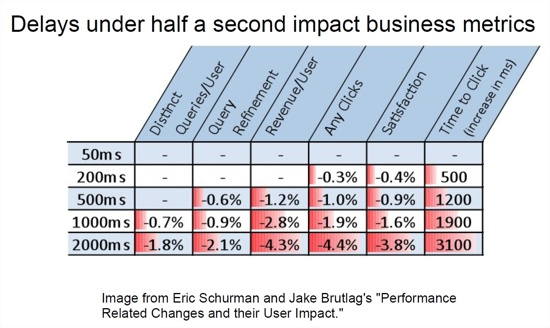
\includegraphics[width=\linewidth]{Resources/LoadTimeDelaysUserImpact.jpg}}};
%   \caption{Laadtijd vertragingen met impact, Bron:~\textcite{McGee2010}}
%   \label{fig:loadTimeDelaysUserImpact}
%   \end{figure}
%

\chapter{\IfLanguageName{dutch}{Inleiding}{Introduction}}
\label{ch:inleiding}

% NEEDS REFACTOR!
De inleiding van deze scriptie bevat de probleemstelling dat als grondlegging dient voor het onderzoek en de verscheidene onderzoeksvragen die hierbij aan bod komen. Verder worden enkele begrippen uitgeklaard die essentieel zijn voor het doornemen van de scriptie.\\

\section{\IfLanguageName{dutch}{Context}{Context}}
\label{sec:context}

Technologie wordt sneller en complexer doorheen de jaren, wat aan de basis ligt voor de snelle evolutie van het web en de hogere standaarden die het teweeg brengt in web uitwerkingen. Dit staat tevens in lineair verband met de moeilijkheidsgraad voor het opleveren van performante en robuuste webapplicaties. \\
De frontend van dergelijke applicaties dient te voldoen aan de snelheid die gebruikers verwachten wanneer ze het \gls{www} betreden. Om dit te verzekeren wordt er aan \emph{performantie optimalisatie} gedaan, door onderzoek te voeren naar specifieke maatstaven en deze te optimaliseren.

\subsection{\IfLanguageName{dutch}{Performantie}{Performance}}
\label{sec:performantie}

Tegenwoordig hoort een robuuste webapplicatie tot elke business van een bedrijf. Het creëert business-waarde door mensen in contact te brengen met de core-business en missie van het bedrijf. Met alle technologische vooruitgang die onze samenleving kende op korte tijd liggen de verwachtingen van mensen ook sneller veel hoger dan daarvoor. De performantie van een webapplicatie komt als goede maatstaf voor hoe zeer het kan voldoen aan die hoge verwachtingen. \\
Uiteindelijk is performantie relatief voor dat geen waar in geïnvesteerd wordt vanuit een business standpunt en hoe het meer waarde kan creëren. De meeste problemen bij gebruikers komen neer op performantie. Bij voorkeur hebben webapplicatie een laadtijd van 0 seconden, wat onmogelijk te bereiken is, maar uiteindelijk is dit wel wat de gebruiker verwacht. Trage laadtijden kunnen een slecht reagerende \gls{ui} opleveren, wat op zich dan ongewenst gedrag oplevert. \\ Performantie is het geheel van al die factoren dat een webapplicatie aanvaardbaar maakt voor de gebruiker. Het komt er op neer dat een business onderzoek doet naar de performantie metrieken waar het in wilt investeren. Dergelijk onderzoek kan ten koste zijn van andere performantie factoren, maar die kost wil men dragen als het een performantie verbetering kan teweeg brengen.

\subsection{\IfLanguageName{dutch}{Beschrijvende metrieken}{Descriptive metrics}}
\label{sec:beschrijvendeMetrieken}

Performantie is geen enkelvoudig begrip. Het definieert een samenhang van metrieken die elk deel bepalen van hoe performant een webapplicatie is. Zoals eerder aangehaald is performantie relatief tot de investering en belangrijkheid voor de business. \\
Er wordt een onderverdeling gedaan tussen de metrieken die performantie definiëren en dit op basis van hun aard. Metrieken kunnen kwalitatief of kwantitatief de performantie gaan voorstellen. In het geval van kwaliteit gaat dat voornamelijk in op de perceptie van een gebruiker die de applicatie gebruikt. Het is niet meetbaar en relatief te opzichte van de omgeving en toestand waarin ze de applicatie gebruiken. Bijvoorbeeld gebruikers die testen met een slechte internet verbinding zullen de applicatie aanvoelen als traag. Ligt dit dan aan het netwerk of andere misschien interne factoren? Dat zijn problemen die gemeten moeten worden. \\
Kwantitatieve metrieken geven de performantie weer in een meetbare eenheid, voornamelijk in functie van tijd en bijhorend uitgedrukt in milliseconden (ms) of seconden (s).

* Quantitive performance indicators
Response time | Throughput (requests per second) | System availability | Responsiveness (in correlation with response time) | Request rate (number of HTTP requests) | Resource consumption (important for good response time and throughput) | Latency (min time to get any sort of response) | Server response (for loading initial HTML for rendering the page)

Er zijn enkel een handvol performantie factoren waar front end ontwikkelaars invloed op kunnen hebben.
% KPI's subsection?

\subsection{\IfLanguageName{dutch}{Optimalisatie}{Optimization}}
\label{sec:optimalisatie}



\subsection{\IfLanguageName{dutch}{Problematiek en testen}{Problems and testing}}
\label{sec:problemen&testen}



\section{\IfLanguageName{dutch}{Probleemstelling}{Problem Statement}}
\label{sec:probleemstelling}

React code bases zijn niet performant op zichzelf, door onderzoek van eigen code base kunnen de juiste methoden toegepast worden waar nodig. Het framework is van zichzelf uit reeds opmerkelijk performant, wat niet wilt zeggen dat projecten uitgewerkt met een React-gebaseerde \emph{tech stack} meteen ook performante uitwerkingen zijn. Door voldoende begrip vergaard te hebben in verband met functionaliteiten die React en samenhangende libraries bieden kan een performante frontend ontwikkeling bekomen worden. \\
Deze scriptie formuleert een bundel van technieken en methodologieën voor performantie optimalisatie op frontend niveau. Het onderzoek is gevoerd vanuit een performantie perspectief met een diepgaande kijk op de werking van React, zowel boven- als onderliggend. Zowel zelfstandig als binnen een onderneming is dit een toevoeging aan ieders frontend React development.

\section{\IfLanguageName{dutch}{Korte Toenadering van het werk}{Brief approach}}
\label{sec:korteToenadering}

% Mention that we only go in on those metrics that we can influence as developers on front end side. Make the link to react and address the way of working

\section{\IfLanguageName{dutch}{Opzet van deze bachelorproef}{Structure of this bachelor thesis}}
\label{sec:opzetBachelorproef}

De rest van deze bachelorproef is als volgt opgebouwd:

In Hoofdstuk~\ref{ch:react} wordt React ontleed voor een goed begrip te krijgen van het framework zelf.

% In Hoofdstuk~\ref{ch:theoretischePerformantie} komt het theoretische aspect van de performantie in kaart en worden de metrieken uitbundig besproken. 

% In Hoofdstuk~\ref{ch:praktischePerformantie} wordt het praktische van performantie op basis van de meest courante technieken uitgewerkt.

% In Hoofdstuk~\ref{ch:conclusie}, tenslotte, wordt de conclusie gegeven en een antwoord geformuleerd op de onderzoeksvragen. Daarbij wordt ook een aanzet gegeven voor toekomstig onderzoek binnen dit domein.